\documentclass{article}
\usepackage{listings}
\usepackage{graphicx}
\usepackage{float}
\usepackage{fontspec}
\setsansfont{Ubuntu}% Ubuntu as sans - use \sffamily or \textsf{} as normal
\setmonofont{JetBrainsMono Nerd Font Mono}% Ubuntu Mono as 'typewriter' - use \ttfamily or \texttt{}
\usepackage[a4paper,
            bindingoffset=0.2in,
            left=1cm,
            right=1cm,
            top=1in,
            bottom=1in,
            footskip=.25in]{geometry}
\usepackage{hyperref}
\hypersetup{
    colorlinks, citecolor=black, filecolor=black,
    linkcolor=black, urlcolor=black
}
\usepackage{xcolor}
\definecolor{mygreen}{rgb}{0.05,0.15,0.11}
\definecolor{mygray}{rgb}{0.9,0.9,0.9}
\definecolor{mymauve}{rgb}{0.58,0,0.82}
\lstset{
  % backgroundcolor=\color{mygray}, 
  basicstyle=\ttfamily,
  breakatwhitespace=false,
  breaklines=true,
  % commentstyle=\color{darkgray},
  keepspaces=true,
  keywordstyle=\bfseries,
  morekeywords={*,...},
  showspaces=false,
  showstringspaces=false,
  showtabs=false,
  % stringstyle=\color{blue},
  tabsize=4,
  % numbers=left,
  rulecolor=\color{black},
  postbreak=\mbox{\textcolor{red}{$\hookrightarrow$}\space}
}

\begin{document}

\pagenumbering{gobble}
{\centerline{\bfseries \Huge Assignment 5}}

\section*{Question 1}
Write a JavaScript function to chop a string into chunks of a given length\\
\textbf{Test Data :}
\begin{lstlisting}
    console.log(string_chop('welcome'));
    console.log(string_chop('welcome',2));
    console.log(string_chop('welcome',3));
Output:
    ["welcome"]
    ["we", "lc", "om", "e"]
    ["wel", "com", "e"]
\end{lstlisting}
\subsection*{Code}
\lstinputlisting[language=html]{1/index.html}
\newpage
\subsection*{Output}
\begin{figure}[H]
  \centering
  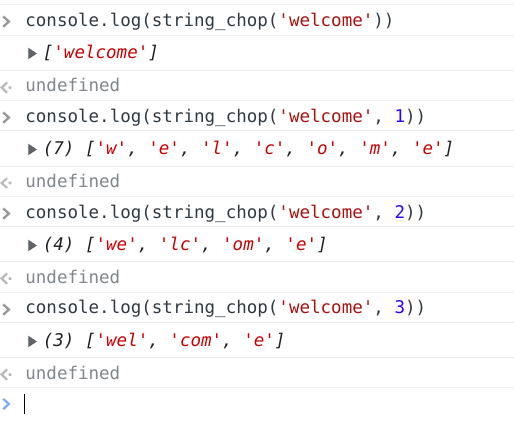
\includegraphics[width=10cm]{1/out.png}
\end{figure}

\newpage
\section*{Question 2}
Write a JavaScript function to convert a string to title case. \\
\textbf{Test Data :}
\begin{lstlisting}
    console.log(sentenceCase('hoW aRe YOU'));
Output:
    "How Are You"
\end{lstlisting}
\subsection*{Code}
\lstinputlisting[language=html]{2/index.html}
\newpage
\subsection*{Output}
\begin{figure}[H]
  \centering
  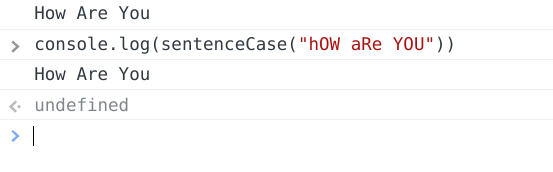
\includegraphics[width=10cm]{2/out.png}
\end{figure}

\newpage
\section*{Question 3}
An Evil number is a positive whole number which has even number of 1's in
it's binary equivalent. \\
Example: 9 - 1001, contains even no of 1's. Thus 9 is evil number.
Design a program to accept a positive whole number $n$ where $n > 2$ and $n < 100$,
and find if the number is evil or not.
\subsection*{Code}
\lstinputlisting[language=html]{3/index.html}
\newpage
\subsection*{Output}
\begin{figure}[H]
  \centering
  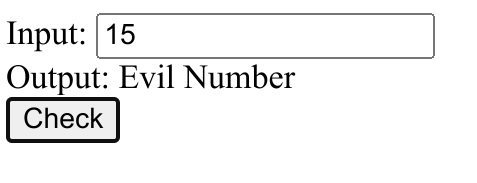
\includegraphics[width=10cm]{3/out.png}
\end{figure}
\end{document}